\documentclass[11pt,titlepage]{article}

\usepackage{geometry}
\usepackage{float}
\usepackage{graphicx}
\geometry{a4paper}
\geometry{margin=2cm}
\geometry{portrait}

\newcommand{\horrule}[1]{\rule{\linewidth}{#1}}

\title{
		\normalfont \normalsize \textsc{COS 330} \\
		%\normalfont \normalsize \textsc{Project Name: KinderFinder} \\ [25pt]
		\horrule{0.5pt} \\[0.4cm]
		\huge Practical 3\\
		\horrule{2pt} \\[0.5cm]
}
\author{\begin{tabular}{rl}
	\texttt{Student Name:} & \texttt{} \\[0.5cm]
	Uteshlen Nadesan & 28163304 \\
\end{tabular}
	\\ \\ \texttt{Version: 0.1}
%	\\ \\ \texttt{Change History:}
%	\\ The Summary here.
	}
\date{14/09/2014} 

\begin{document}
\maketitle
\tableofcontents
\newpage

\section{Task 1}
Find the password hash for the root account on your Kali Linux virtual machine (hint  -look  at  '/etc/shadow'  as  root).  Place  the  hash  in  your  own  file  (hint  -  consult  online 
documentation for shadow file format and look in '/etc/login.defs'). Use hashcat to bruteforce  the  password  (hint  -  use  'hashcat  -h'  and  online  documentation).  Provide  the 
following for your answer:
\subsection{Hash type used by Kali Linux. [1]}
Hashtype : SHA-512

\subsection{Hashcat command line with parameters used. [4]}
\begin{figure}[H]
\begin{center}
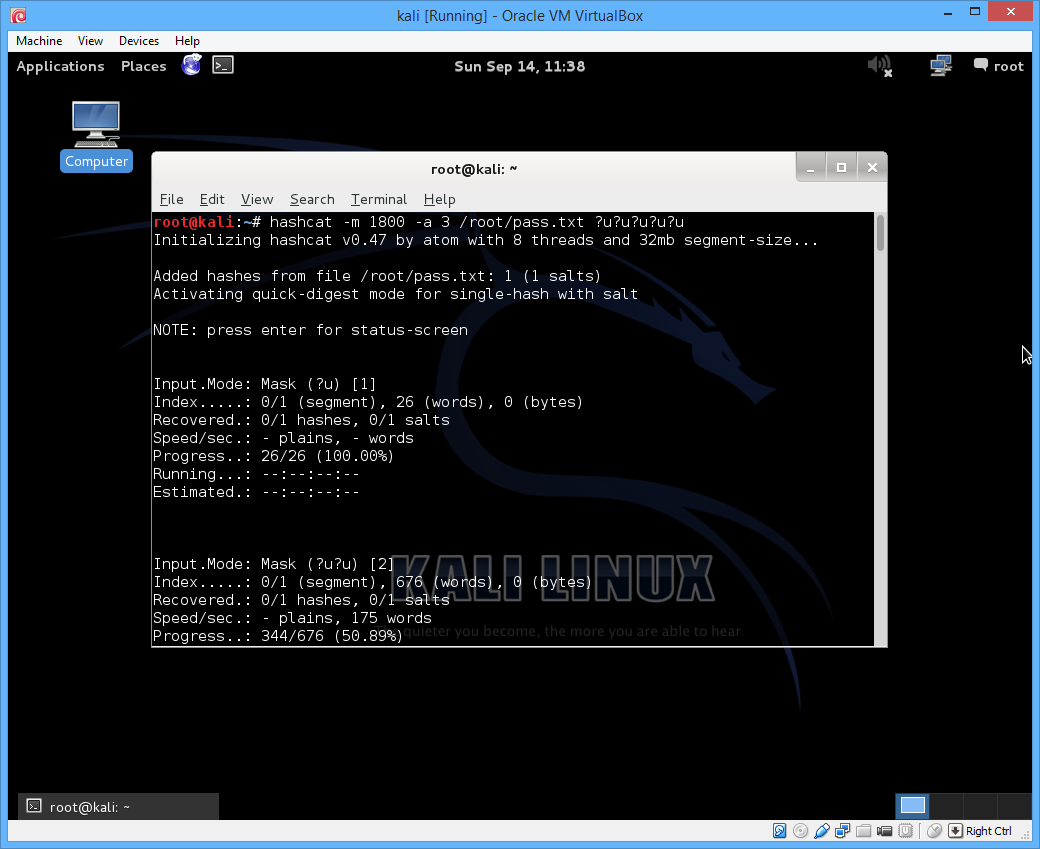
\includegraphics[scale=0.6]{task1b.png}
\caption{task 1b}
\end{center}
\end{figure}

\subsection{Screenshot  of  hashcat  clearly  showing  the  retrieved  password  (root)  and  time elapsed. [2]}

\begin{figure}[H]
\begin{center}
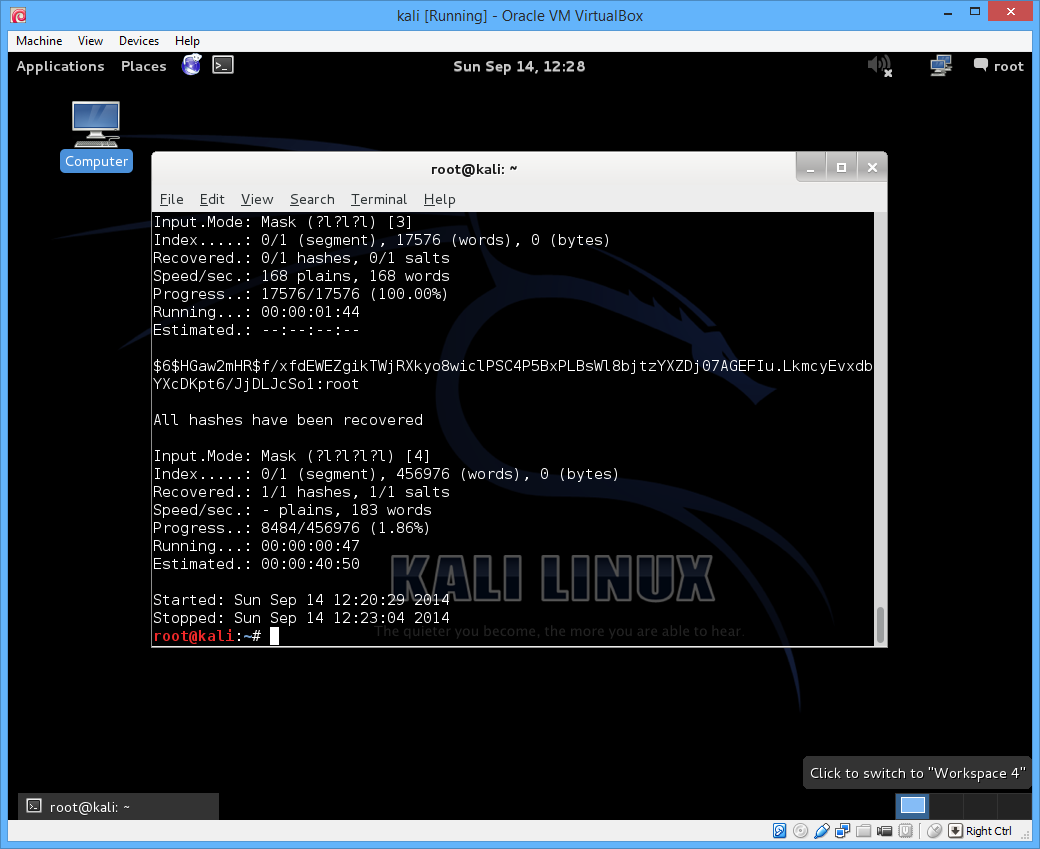
\includegraphics[scale=0.6]{task1c.png}
\caption{task 1c}
\end{center}
\end{figure}

\section{Task 2}
Now use hashcat on the password hash of your own account. Show that the chosen 
password is weak if the format is known. Provide the following for your answer:
\subsection{Hashcat command line with parameters used. [4]}
\begin{figure}[H]
\begin{center}
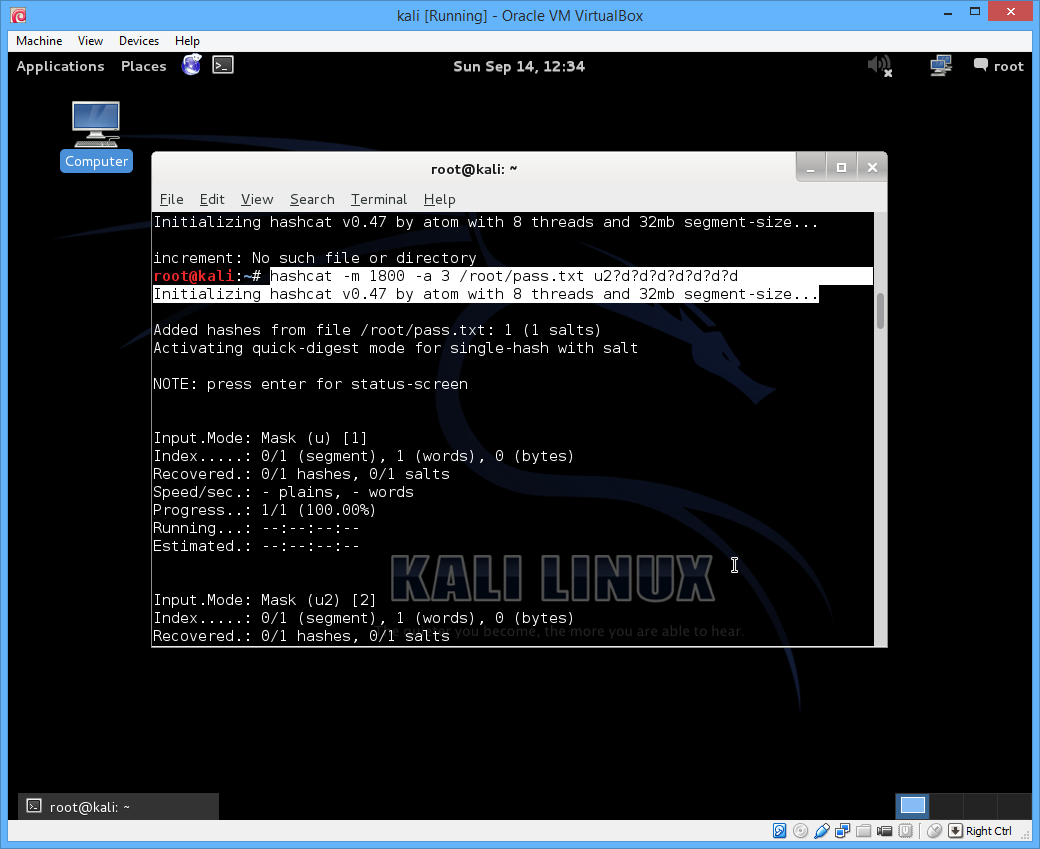
\includegraphics[scale=0.6]{task2a.png}
\caption{task 2a}
\end{center}
\end{figure}

\subsection{Screenshot of hashcat running (status) with time left estimation. [2]}
\begin{figure}[H]
\begin{center}
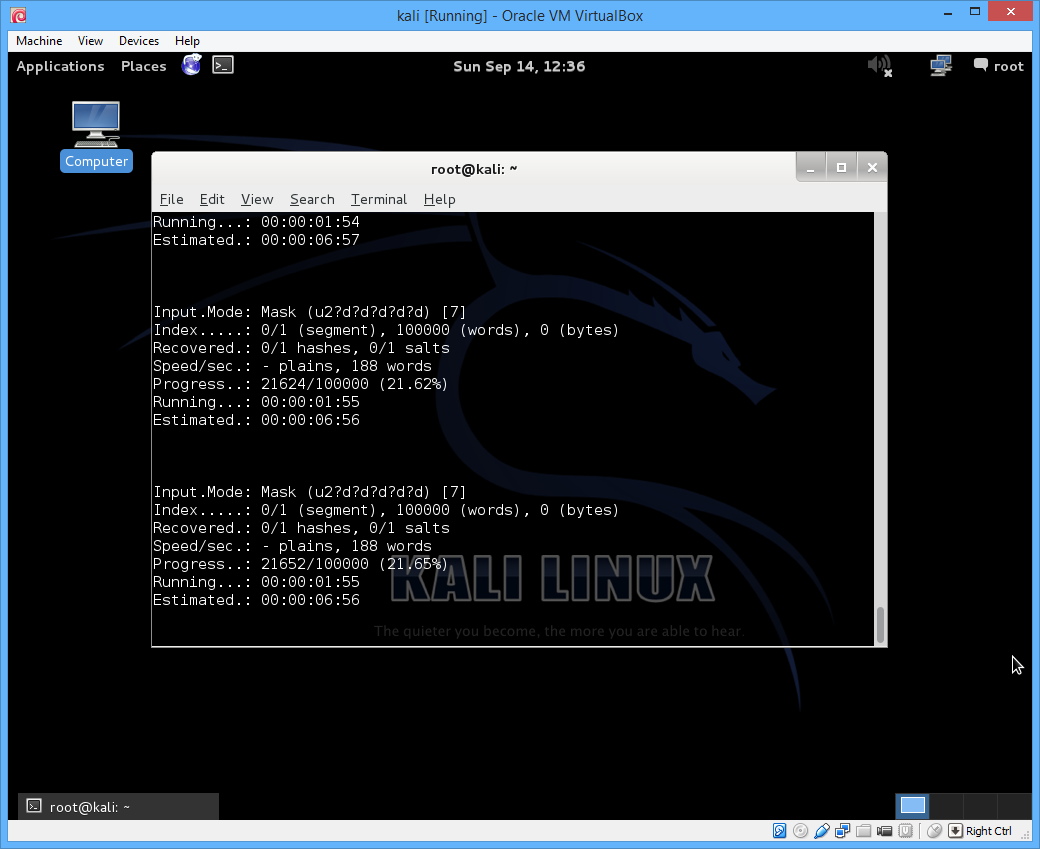
\includegraphics[scale=0.6]{task2b.png}
\caption{task 2b - running}
\end{center}
\end{figure}

\begin{figure}[H]
\begin{center}
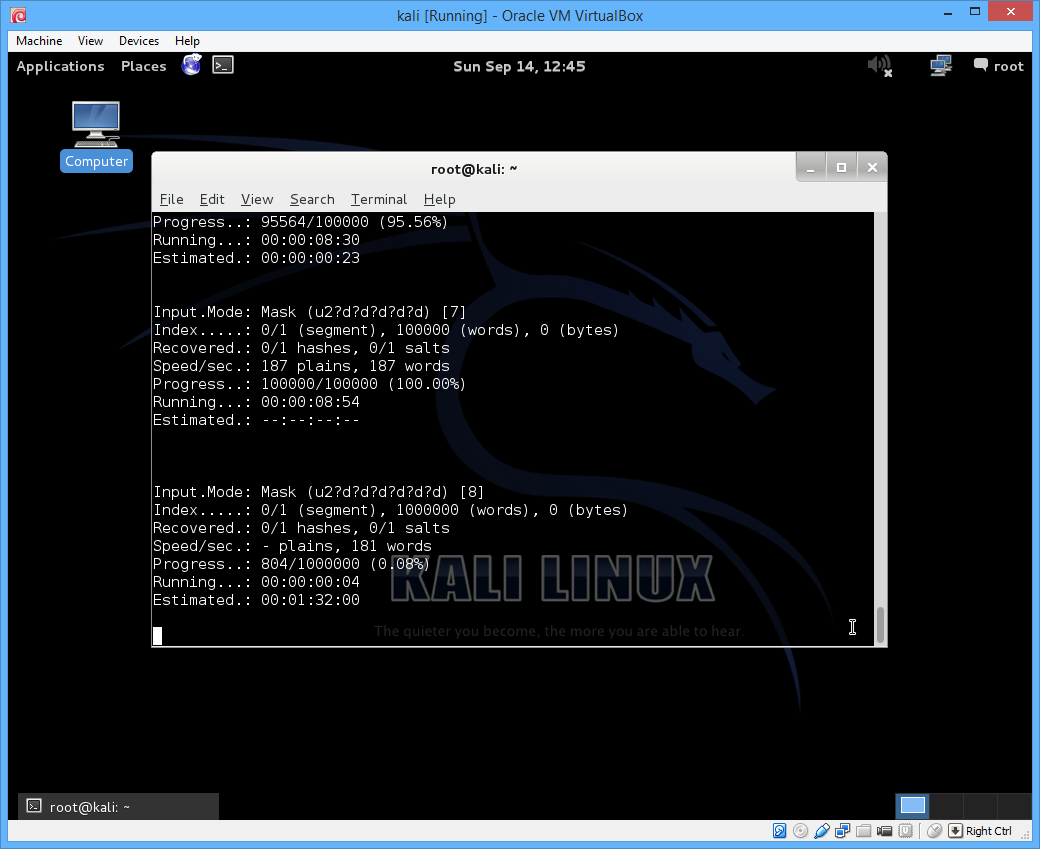
\includegraphics[scale=0.6]{task2b2.png}
\caption{task 2b - running}
\end{center}
\end{figure}

\section{Task 3}
Change  your  password  to  a  strong  password.  Use  hashcat  to  prove  the  password  is strong. Provide the following for your answer:
\subsection{Your chosen password. [1]}
Chosen Password: F@.k3pSW*d!171
\subsection{Hashcat command line with parameters used. [4]}
\begin{figure}[H]
\begin{center}
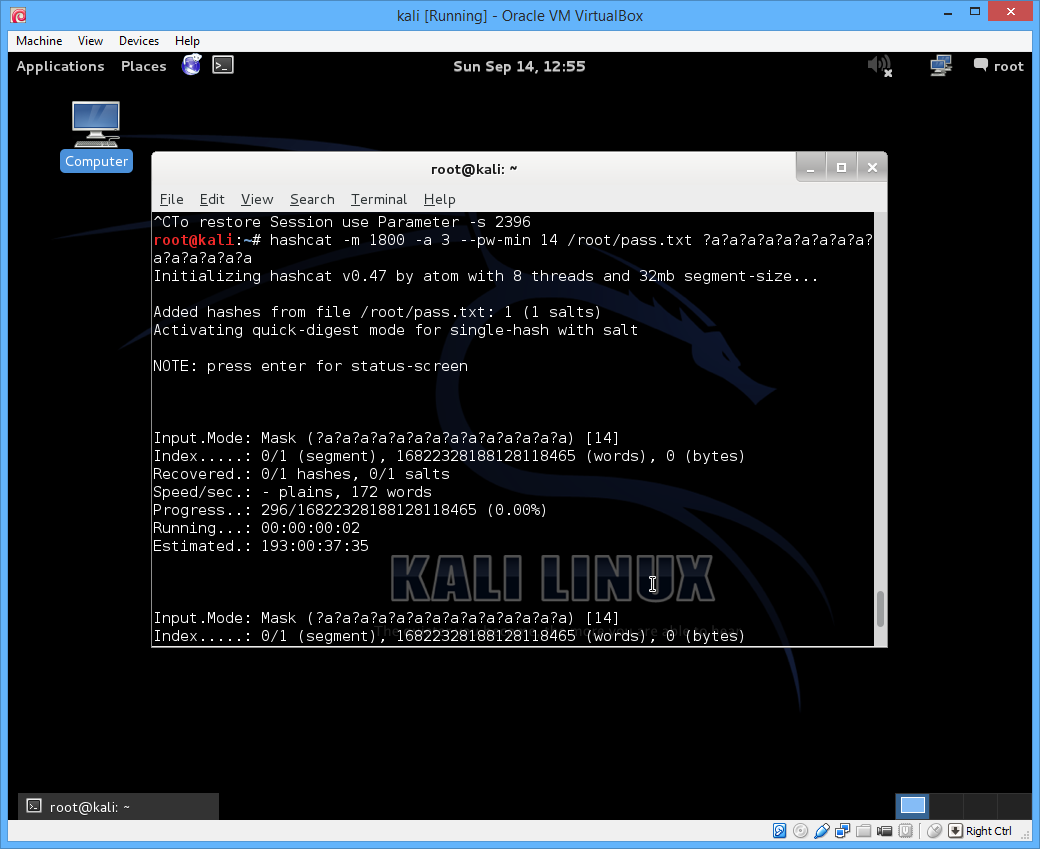
\includegraphics[scale=0.6]{task3b.png}
\caption{task 3b}
\end{center}
\end{figure}

\subsection{Screenshot of hashcat running (status) with time left estimation. [2]}
\begin{figure}[H]
\begin{center}
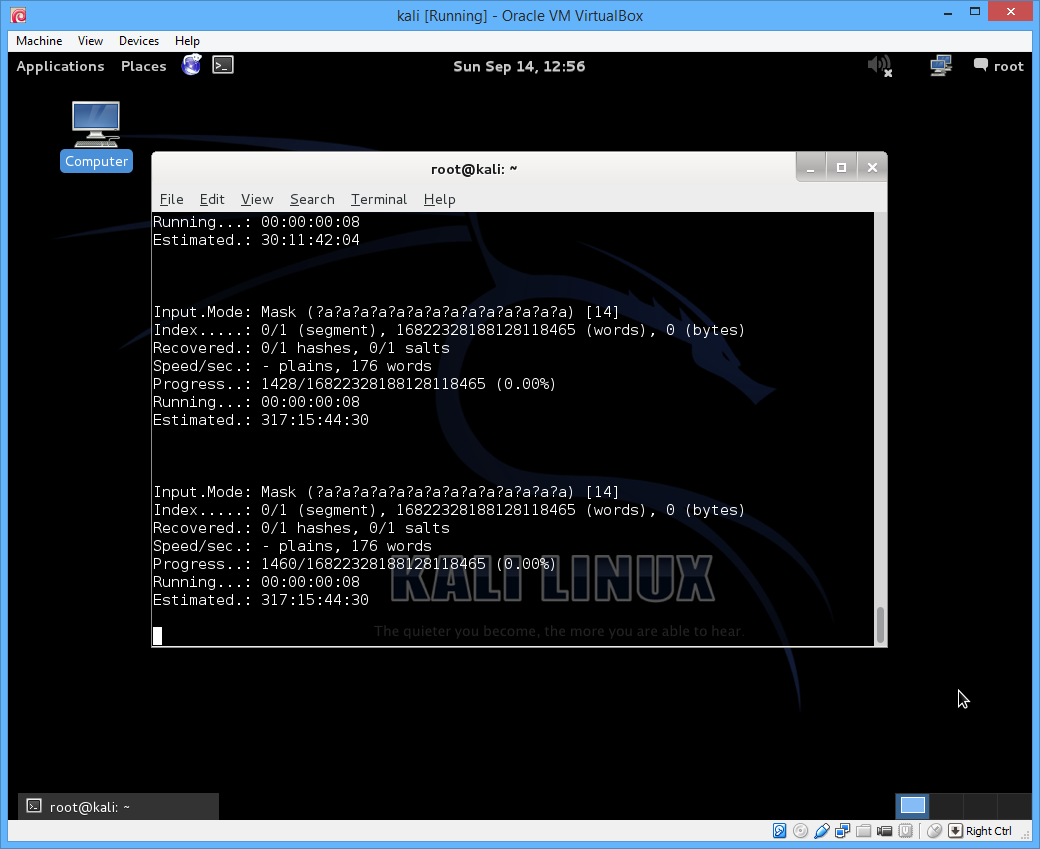
\includegraphics[scale=0.6]{task3c.png}
\caption{task3c}
\end{center}
\end{figure}
%\begin{figure}[H]
%\begin{center}
%\includegraphics[scale=0.8]{SystemArchitecture.jpg}
%\caption{System architecture.}
%\end{center}
%\end{figure}
\end{document}

